\documentclass[../main.tex]{subfiles}

\setcounter{section}{5}

\begin{document}

    \thispagestyle{1page}
    
    \section[Separation in the Vicinity of Aerodromes]{\texorpdfstring{SEPARATION IN THE VICINITY OF AERODROMES}{}}

    \subsection[Reduction in separation minima in the vicinity of aerodromes]{REDUCTION IN SEPARATION MINIMA IN \\ THE VICINITY OF AERODROMES}

    %References
    In addition to the circumstances mentioned in Chapter 5, 5.11.1, the separation minima detailed in Chapter 5, 5.4.1 and 5.4.2, may be reduced in the vicinity of aerodromes if:

    \begin{enumalph}
        \item adequate separation can be provided by the aerodrome controller when each aircraft is continuously visible to this controller; or
        \item each aircraft is continuously visible to flight crews of the other aircraft concerned and the pilots thereof report that they can maintain their own separation; or
        \item in the case of one aircraft following another, the flight crew of the succeeding aircraft reports that the other aircraft is in sight and separation can be maintained.
    \end{enumalph}

    \subsection[Essential local traffic]{ESSENTIAL LOCAL TRAFFIC}

    \begin{enumerate}[label=\arabic{section}.\arabic{subsection}.\arabic*]
        \item Information on essential local traffic known to the controller shall be transmitted without delay to departing and arriving aircraft concerned.

        \note[1]{Essential local traffic in this context consists of any aircraft, vehicle or personnel on or near the runway to be used, or traffic in the take-off and climb-out area or the final approach area, which may constitute a collision hazard to a departing or arriving aircraft.}

        %References
        \note[2]{See also Chapter 5, Section 5.10, Chapter 7, 7.4.1.3 and Chapter 8, 8.8.2.}

        \begin{enumerate}[label=\arabic{section}.\arabic{subsection}.\arabic{enumi}.\arabic*]
            \item Essential local traffic shall be described so as to be easily identified.
        \end{enumerate}
    \end{enumerate}

    \subsection[Procedures for departing aircraft]{PROCEDURES FOR DEPARTING AIRCRAFT}

    \subsubsection{General}

    \begin{enumerate}
        \item Clearances for departing aircraft shall specify, when necessary for the separation of aircraft, direction of take-off and turn after take-off; heading or track to be made good before taking up the cleared departure track; level to maintain before continuing climb to assigned level; time, point and/or rate at which a level change shall be made; and any other necessary manoeuvre consistent with safe operation of the aircraft.
        \item At aerodromes where standard instrument departures (SIDs) have been established, departing aircraft should normally be cleared to follow the appropriate SID.
    \end{enumerate}

    \subsubsection{Standard clearances for departing aircraft}

    \begin{enumerate}[itemsep=0.2cm]\centering
        \item \textsc{General}
        \begin{enumempty}
            \item The appropriate ATS authority should, wherever possible, establish standardized procedures for transfer of control between the ATC units concerned, and standard clearances for departing aircraft.

            %References
            \note{The provisions applying to standardized procedures for coordination and transfer of control are specified in Chapter 10, Section 10.1.1.}
        \end{enumempty}

        \item \textsc{Coordination}
        \begin{enumerate}
            \item Where standard clearances for departing aircraft have been agreed to between the units concerned, the aerodrome control tower will normally issue the appropriate standard clearance without prior coordination with or approval from the approach control unit or ACC.
            \item Prior coordination of clearances should be required only in the event that a variation to the standard clearance or the standardized transfer of control procedures is necessary or desirable for operational reasons.
            \item Provision shall be made to ensure that the approach control unit at all times is kept informed of the sequence in which aircraft will depart as well as the runway to be used.
            \item Provision shall be made to display the designators of assigned SIDs to the aerodrome control tower, the approach control unit and/or the ACC as applicable.
        \end{enumerate}

        \item \textsc{Contents}
        \begin{enumempty}
            \item Standard clearances for departing aircraft shall contain the following items:
        \end{enumempty}
        \begin{enumalph}
            \item aircraft identification;
            \item clearance limit, normally destination aerodrome;
            \item designator of the assigned SID, if applicable;
            \item cleared level;
            \item allocated SSR code;
            \item any other necessary instructions or information not contained in the SID description, e.g. instructions relating to change of frequency.
        \end{enumalph}
        \begin{enumempty}[labelindent=\parindent]
            \item \note[1]{See \ref{6.3.2.4.1} for clearances to aircraft on SID.}

            \item \note[2]{The use of a SID designator without a cleared level does not authorize the aircraft to climb on the SID vertical profile.}
        \end{enumempty}

        \item \textsc{Clearances on a SID}
        \begin{enumerate}
            \item \label{6.3.2.4.1} Clearances to aircraft on a SID with remaining published level and/or speed restrictions shall indicate if such restrictions are to be followed or are cancelled. The following phraseologies shall be used with the following meanings:

            \begin{enumalph}
                \item CLIMB VIA SID TO \textit{(level)}:
                \begin{enumerate}[label=\roman*),labelsep=0.1cm,leftmargin=*,parsep=0pt]
                    \item climb to the cleared level and comply with published level restrictions;
                    \item follow the lateral profile of the SID; and
                    \item comply with published speed restrictions or ATC-issued speed control instructions as applicable.
                \end{enumerate}

                \item CLIMB VIA SID TO \textit{(level)}, CANCEL LEVEL RESTRICTION(S):
                \begin{enumerate}[label=\roman*),labelsep=0.1cm,leftmargin=*,parsep=0pt]
                    \item climb to the cleared level; published level restrictions are cancelled;
                    \item follow the lateral profile of the SID; and
                    \item comply with published speed restrictions or ATC-issued speed control instructions as applicable.
                \end{enumerate}

                \item CLIMB VIA SID TO \textit{(level)}, CANCEL LEVEL RESTRICTION(S) AT \textit{(point(s))}:
                \begin{enumerate}[label=\roman*),labelsep=0.1cm,leftmargin=*,parsep=0pt]
                    \item climb to the cleared level; published level restriction(s) at the specified point(s) are cancelled;
                    \item follow the lateral profile of the SID; and
                    \item comply with published speed restrictions or ATC-issued speed control instructions as applicable.
                \end{enumerate}

                \item CLIMB VIA SID TO \textit{(level)}, CANCEL SPEED RESTRICTION(S):
                \begin{enumerate}[label=\roman*),labelsep=0.1cm,leftmargin=*,parsep=0pt]
                    \item climb to the cleared level and comply with published level restrictions;
                    \item follow the lateral profile of the SID; and
                    \item published speed restrictions and ATC-issued speed control instructions are cancelled.
                \end{enumerate}

                \item CLIMB VIA SID TO \textit{(level)}, CANCEL SPEED RESTRICTION(S) AT \textit{(point(s))}:
                \begin{enumerate}[label=\roman*),labelsep=0.1cm,leftmargin=*,parsep=0pt]
                    \item climb to the cleared level and comply with published level restrictions;
                    \item follow the lateral profile of the SID; and
                    \item published speed restrictions are cancelled at the specified point(s).
                \end{enumerate}

                \item CLIMB UNRESTRICTED TO \textit{(level)} or CLIMB TO \textit{(level)}, CANCEL LEVEL AND SPEED RESTRICTION(S):
                \begin{enumerate}[label=\roman*),labelsep=0.1cm,leftmargin=*,parsep=0pt]
                    \item climb to the cleared level; published level restrictions are cancelled;
                    \item follow the lateral profile of the SID; and
                    \item published speed restrictions and ATC-issued speed control instructions are cancelled.
                \end{enumerate}
            \end{enumalph}

            \item If there are no remaining published level or speed restrictions on the SID, the phrase CLIMB TO \textit{(level)} should be used.
            \item When subsequent speed restriction instructions are issued, and if the cleared level is unchanged, the phrase CLIMB VIA SID TO \textit{(level)} should be omitted.
            \item When a departing aircraft is cleared to proceed direct to a published waypoint on the SID, the speed and level restrictions associated with the bypassed waypoints are cancelled. All remaining published speed and level restrictions shall remain applicable.
            \item \label{6.3.2.4.5} When a departing aircraft is vectored or cleared to proceed to a point that is not on the SID, all the published speed and level restrictions of the SID are cancelled and the controller shall:

            \begin{enumalph}
                \item reiterate the cleared level;
                \item provide speed and level restrictions as necessary; and
                \item notify the pilot if it is expected that the aircraft will be instructed to subsequently rejoin the SID.
            \end{enumalph}
            
            %References
            \note{See also 8.6.5.2 regarding prescribed obstacle clearance.}

            \item ATC instructions to an aircraft to rejoin a SID shall include:

            \begin{enumalph}
                \item the designator of the SID to be rejoin, unless advance notification of rejoin has been provided in accordance with \ref{6.3.2.4.5};
                \item the cleared level in accordance with \ref{6.3.2.4.1}; and
                \item the position at which it is expected to rejoin the SID.
            \end{enumalph}
            
            %References
            \note{See 12.3.3.1 for phraseology on rejoin instructions.}
            
        \end{enumerate}

        \item \textsc{Communication failure}

        \begin{enumerate}
            \item Clearances for departing aircraft may specify a cleared level other than that indicated in the filed flight plan for the en-route phase of flight, without a time or geographical limit for the cleared level. Such clearances will normally be used to facilitate the application of tactical control methods by ATC, normally through the use of an ATS surveillance system.
            \item Where clearances for departing aircraft contain no time or geographical limit for a cleared level, action to be taken by an aircraft experiencing air-ground communication failure in the event the aircraft has been radar vectored away from the route specified in its current flight plan should be prescribed on the basis of a regional air navigation agreement and included in the SID description or published in AIPs.
        \end{enumerate}
    \end{enumerate}

    \subsubsection{Departure sequence}

    \begin{enumerate}
        \item Departing aircraft may be expedited by suggesting a take-off direction which is not into the wind. It is the responsibility of the pilot-in-command of an aircraft to decide between making such a take-off or waiting for take-off in a preferred direction.
        \item If departures are delayed, the delayed flights shall normally be cleared in an order based on their estimated time of departure, except that deviation from this order may be made to:

        \begin{enumalph}
            \item facilitate the maximum number of departures with the least average delay;
            \item accommodate requests by an operator in respect of that operator’s flights to the extent practicable.
        \end{enumalph}

        \item Air traffic control units should, when practicable, advise aircraft operators or their designated representatives when anticipated delays are expected to exceed 30 minutes.
    \end{enumerate}

    \subsection[Information for departing aircraft]{INFORMATION FOR DEPARTING AIRCRAFT}

    \begin{enumempty}[labelindent=\parindent]
        %References
        \item \note{See Chapter 11, 11.4.3, regarding flight information messages.}
    \end{enumempty}

    \subsubsection{Meteorological conditions}

    Information regarding significant changes in the meteorological conditions in the take-off or climb-out area, obtained by the unit providing approach control service after a departing aircraft has established communication with such unit, shall be transmitted to the aircraft without delay, except when it is known that the aircraft already has received the information.

    \note{Significant changes in this context include those relating to surface wind direction or speed, visibility, runway visual range or air temperature (for turbine-engined aircraft), and the occurrence of thunderstorm or cumulonimbus, moderate or severe turbulence, wind shear, hail, moderate or severe icing, severe squall line, freezing precipitation, severe mountain waves, sandstorm, duststorm, blowing snow, tornado or waterspout.}

    \subsubsection{Operational status of visual or non-visual aids}

    Information regarding changes in the operational status of visual or non-visual aids essential for take-off and climb shall be transmitted without delay to a departing aircraft, except when it is known that the aircraft already has received the information.

    \subsection[Procedures for arriving aircraft]{PROCEDURES FOR ARRIVING AIRCRAFT}

    \subsubsection{General}

    \begin{enumerate}
        \item When it becomes evident that delays will be encountered by arriving aircraft, operators or designated representatives shall, to the extent practicable, be notified and kept currently informed of any changes in such expected delays.
        \item Arriving aircraft may be required to report when leaving or passing a significant point or navigation aid, or when starting procedure turn or base turn, or to provide other information required by the controller, to expedite departing and arriving aircraft.
        \item An IFR flight shall not be cleared for an initial approach below the appropriate minimum altitude as specified by the State concerned nor to descend below that altitude unless:

        \begin{enumalph}
            \item the pilot has reported passing an appropriate point defined by a navigation aid or as a waypoint; or
            \item the pilot reports that the aerodrome is and can be maintained in sight; or
            \item the aircraft is conducting a visual approach; or
            \item the controller has determined the aircraft’s position by the use of an ATS surveillance system, and a lower minimum altitude has been specified for use when providing ATS surveillance services.
        \end{enumalph}

        \item At aerodromes where standard instrument arrivals (STARs) have been established, arriving aircraft should normally be cleared to follow the appropriate STAR. The aircraft shall be informed of the type of approach to expect and runway-in-use as early as possible.

        \note{See Section \ref{6.5.2} concerning Standard arrival clearances.}

        \item After coordination with the approach control unit, the ACC may clear the first arriving aircraft for approach rather than to a holding fix.
    \end{enumerate}

    \subsubsection{Standard clearances for arriving aircraft} \label{6.5.2}

    \begin{enumerate}[itemsep=0.2cm]\centering
        \item \textsc{General}
        \begin{enumempty}
            \item The appropriate ATS authority should, wherever possible, establish standardized procedures for transfer of control between the ATC units concerned, and standard clearances for arriving aircraft.

            %References
            \note{The provisions applying to standardized procedures for coordination and transfer of control are specified in Chapter 10, Section 10.1.1.}
        \end{enumempty}

        \item \textsc{Coordination}
        \begin{enumerate}
            \item Where standard clearances for arriving aircraft are in use and, provided no terminal delay is expected,clearance to follow the appropriate STAR will normally be issued by the ACC without prior coordination with or approval from the approach control unit or the aerodrome control tower as applicable.
            \item Prior coordination of clearances should be required only in the event that a variation to the standard clearance or the standardized transfer of control procedures is necessary or desirable for operational reasons.
            \item Provision shall be made to ensure that the approach control unit is at all times kept informed of the sequence of aircraft following the same STAR.
            \item Provision shall be made to display the designators of assigned STARs to the ACC, the approach control unit and/or the aerodrome control tower, as applicable.
        \end{enumerate}

        \item \textsc{Contents}
        \begin{enumempty}
            \item Standard clearances for arriving aircraft shall contain the following items:
            \begin{enumalph}
                \item aircraft identification;
                \item designator of the assigned STAR if applicable;
                \item runway-in-use, except when part of the STAR description;
                \item cleared level; and
                \item any other necessary instructions or communications.
            \end{enumalph}

            \note[1]{See \ref{6.5.2.4.1} for clearances on a STAR.}

            \note[2]{The use of a STAR designator without a cleared level does not authorize the aircraft to descend on the STAR vertical profile.}
        \end{enumempty}

        \item \textsc{Clearances on a STAR}
        \begin{enumerate}
            \item \label{6.5.2.4.1} Clearances to aircraft on a STAR with remaining published level and/or speed restrictions shall indicate if such restrictions are to be followed or are cancelled. The following phraseologies shall be used with the following meaning:
        
            \begin{enumalph}
                \item DESCEND VIA STAR TO \textit{(level)}:
                \begin{enumerate}[label=\roman*),labelsep=0.1cm,leftmargin=*,parsep=0pt]
                    \item descend to the cleared level and comply with published level restrictions;
                    \item follow the lateral profile of the STAR; and
                    \item comply with published speed restrictions or ATC-issued speed control instructions as applicable.
                \end{enumerate}

                \item DESCEND VIA STAR TO \textit{(level)}, CANCEL LEVEL RESTRICTION(S):
                \begin{enumerate}[label=\roman*),labelsep=0.1cm,leftmargin=*,parsep=0pt]
                    \item descend to the cleared level; published level restrictions are cancelled;
                    \item follow the lateral profile of the STAR; and
                    \item comply with published speed restrictions or ATC-issued speed control instructions as applicable.
                \end{enumerate}

                \item DESCEND VIA STAR TO \textit{(level)}, CANCEL LEVEL RESTRICTION(S) AT \textit{(point(s))}:
                \begin{enumerate}[label=\roman*),labelsep=0.1cm,leftmargin=*,parsep=0pt]
                    \item descend to the cleared level; published level restriction(s) at the specified point(s) are cancelled;
                    \item follow the lateral profile of the STAR; and
                    \item comply with published speed restrictions or ATC-issued speed control instructions as applicable.
                \end{enumerate}

                \item DESCEND VIA STAR TO \textit{(level)}, CANCEL SPEED RESTRICTION(S):
                \begin{enumerate}[label=\roman*),labelsep=0.1cm,leftmargin=*,parsep=0pt]
                    \item descend to the cleared level and comply with published level restrictions;
                    \item follow the lateral profile of the STAR; and
                    \item published speed restrictions and ATC-issued speed control instructions are cancelled.
                \end{enumerate}

                \item DESCEND VIA STAR TO \textit{(level)}, CANCEL SPEED RESTRICTION(S) AT \textit{(point(s))}:
                \begin{enumerate}[label=\roman*),labelsep=0.1cm,leftmargin=*,parsep=0pt]
                    \item descend to the cleared level and comply with published level restrictions;
                    \item follow the lateral profile of the STAR; and
                    \item published speed restrictions are cancelled at the specified point(s).
                \end{enumerate}

                \item DESCEND UNRESTRICTED TO \textit{(level)} or DESCEND TO \textit{(level)}, CANCEL LEVEL AND SPEED RESTRICTION(S):
                \begin{enumerate}[label=\roman*),labelsep=0.1cm,leftmargin=*,parsep=0pt]
                    \item descend to the cleared level; published level restrictions are cancelled;
                    \item follow the lateral profile of the STAR; and
                    \item published speed restrictions and ATC-issued speed control instructions are cancelled.
                \end{enumerate}
            \end{enumalph}

            \item If there are no remaining published level or speed restrictions on the STAR, the phrase DESCEND TO \textit{(level)} should be used.
            \item When subsequent speed restriction instructions are issued and if the cleared level is unchanged, the phrase DESCEND VIA STAR TO \textit{(level)} should be omitted.
            \item When an arriving aircraft is cleared to proceed direct to a published waypoint on the STAR, the speed and level restrictions associated with the bypassed waypoints are cancelled. All remaining published speed and level restrictions shall remain applicable.
            \item \label{6.5.2.4.5} When an arriving aircraft is vectored or cleared to proceed to a point that is not on the STAR, all the published speed and level restrictions of the STAR are cancelled and the controller shall:

            \begin{enumalph}
                \item reiterate the cleared level;
                \item provide speed and level restrictions as necessary; and
                \item notify the pilot if it is expected that the aircraft will be instructed to subsequently rejoin the STAR.
            \end{enumalph}
            
            %References
            \note{See 8.6.5.2 regarding prescribed obstacle clearance.}

            \item ATC instructions to an aircraft to rejoin a STAR shall include:

            \begin{enumalph}
                \item the designator of the STAR to be rejoined, unless advance notification of rejoin has been provided in accordance with \ref{6.5.2.4.5};
                \item the cleared level on rejoining the STAR in accordance with \ref{6.5.2.4.1}; and
                \item the position at which it is expected to rejoin the STAR.
            \end{enumalph}
            
            %References
            \note{See 12.3.3.2 for phraseology on rejoin instructions.}
        \end{enumerate}        
    \end{enumerate}

    \subsubsection{Visual approach}

    \begin{enumerate}
        \item Subject to the conditions in \ref{6.5.3.3}, clearance for an IFR flight to execute a visual approach may be requested by a flight crew or initiated by the controller. In the latter case, the concurrence of the flight crew shall be required.
        \item Controllers shall exercise caution in initiating a visual approach when there is reason to believe that the flight crew concerned is not familiar with the aerodrome and its surrounding terrain. Controllers should also take into consideration the prevailing traffic and meteorological conditions when initiating visual approaches.
        \item \label{6.5.3.3} An IFR flight may be cleared to execute a visual approach provided the pilot can maintain visual reference to the terrain and:

        \begin{enumalph}
            \item the reported ceiling is at or above the level of the beginning of the initial approach segment for the aircraft so cleared; or
            \item the pilot reports at the level of the beginning of the initial approach segment or at any time during the instrument approach procedure that the meteorological conditions are such that with reasonable assurance a visual approach and landing can be completed.
        \end{enumalph}

        \item Separation shall be provided between an aircraft cleared to execute a visual approach and other arriving and departing aircraft.
        \item For successive visual approaches, separation shall be maintained by the controller until the pilot of a succeeding aircraft reports having the preceding aircraft in sight. The aircraft shall then be instructed to follow and maintain own separation from the preceding aircraft. When both aircraft are of a heavy wake turbulence category, or the preceding aircraft is of a heavier wake turbulence category than the following, and the distance between the aircraft is less than the appropriate wake turbulence minimum, the controller shall issue a caution of possible wake turbulence. The pilot-in-command of the aircraft concerned shall be responsible for ensuring that the spacing from a preceding aircraft of a heavier wake turbulence category is acceptable. If it is determined that additional spacing is required, the flight crew shall inform the ATC unit accordingly, stating their requirements.
        \item Transfer of communications to the aerodrome controller should be effected at such a point or time that information on essential local traffic, if applicable, and clearance to land or alternative instructions can be issued to the aircraft in a timely manner.
    \end{enumerate}

    \subsubsection{Instrument approach}

    \begin{enumerate}
        \item The approach control unit shall specify the instrument approach procedure to be used by arriving aircraft. A flight crew may request an alternative procedure and, if circumstances permit, should be cleared accordingly.
        \item If a pilot reports or it is clearly apparent to the ATC unit that the pilot is not familiar with an instrument approach procedure, the initial approach level, the point (in minutes from the appropriate reporting point) at which base turn or procedure turn will be started, the level at which the procedure turn shall be carried out and the final approach track shall be specified, except that only the last-mentioned need be specified if the aircraft is to be cleared for a straight-in approach. The frequency(ies) of the navigation aid(s) to be used as well as the missed approach procedure shall also be specified when deemed necessary.
        \item If visual reference to terrain is established before completion of the approach procedure, the entire procedure must nevertheless be executed unless the aircraft requests and is cleared for a visual approach.
    \end{enumerate}

    \subsubsection{Holding}

    \begin{enumerate}
        \item In the event of extended delays, aircraft should be advised of the anticipated delay as early as possible and, when practicable, be instructed or given the option to reduce speed en route in order to absorb delay.
        \item When delay is expected, the ACC shall normally be responsible for clearing aircraft to the holding fix, and for including holding instructions, and expected approach time or onward clearance time, as applicable, in such clearances. (See Section \ref{6.5.8}.)
        \item After coordination with the approach control unit, the ACC may clear an arriving aircraft to a visual holding location to hold until further advised by the approach control unit.
        \item After coordination with the aerodrome control tower, the approach control unit may clear an arriving aircraft to a visual holding location to hold until further advised by the aerodrome control tower.
        \item Holding and holding pattern entry shall be accomplished in accordance with procedures established by the appropriate ATS authority and published in AIPs. If entry and holding procedures have not been published or if the procedures are not known to a flight crew, the appropriate air traffic control unit shall specify the designator of the location or aid to be used, the inbound track, radial or bearing, direction of turn in the holding pattern as well as the time of the outbound leg or the distances between which to hold.
        \item Aircraft should normally be held at a designated holding fix. The required minimum vertical, lateral or longitudinal separation from other aircraft shall be provided. Criteria and procedures for the simultaneous use of adjacent holding patterns shall be prescribed in local instructions.

        %References
        \note{See Chapter 5, Section 5.5, concerning separation of aircraft holding in flight.}

        \item Levels at a holding fix or visual holding location shall as far as practicable be assigned in a manner that will facilitate clearing each aircraft to approach in its proper priority. Normally, the first aircraft to arrive over a holding fix or visual holding location should be at the lowest level, with following aircraft at successively higher levels.
        \item When extended holding is anticipated, turbojet aircraft should, when practicable, be permitted to hold at higher levels in order to conserve fuel, while retaining their order in the approach sequence.
        \item If an aircraft is unable to comply with the published or cleared holding procedure, alternative instructions shall be issued.
        \item For the purpose of maintaining a safe and orderly flow of traffic, an aircraft may be instructed to orbit at its present or at any other position, provided the required obstacle clearance is ensured.
    \end{enumerate}

    \subsubsection{Approach sequence}

    \begin{enumerate}[itemsep=0.2cm]\centering
        \item \textsc{General}
        \begin{enumempty}
            \item The following procedures shall be applied whenever approaches are in progress.
        \end{enumempty}
        \begin{enumerate}
            \item The approach sequence shall be established in a manner which will facilitate arrival of the maximum number of aircraft with the least average delay. Priority shall be given to:

            \begin{enumalph}
                \item an aircraft which anticipates being compelled to land because of factors affecting the safe operation of the aircraft (engine failure, shortage of fuel, etc.);
                \item hospital aircraft or aircraft carrying any sick or seriously injured person requiring urgent medical attention;
                \item aircraft engaged in search and rescue operations; and
                \item other aircraft as may be determined by the appropriate authority.
            \end{enumalph}

            %References
            \note{An aircraft which has encountered an emergency is handled as outlined in Chapter 15, Section 15.1.}

            \item Succeeding aircraft shall be cleared for approach:

            \begin{enumalph}
                \item when the preceding aircraft has reported that it is able to complete its approach without encountering instrument meteorological conditions; or
                \item when the preceding aircraft is in communication with and sighted by the aerodrome control reasonable assurance exists that a normal landing can be accomplished; or
                \item when timed approaches are used, the preceding aircraft has passed the defined point inbound, and reasonable assurance exists that a normal landing can be accomplished;

                \note{See \ref{6.5.6.2.1} concerning timed approach procedures.}

                \item when the use of an ATS surveillance system confirms that the required longitudinal spacing between succeeding aircraft has been established.
            \end{enumalph}

            \item In establishing the approach sequence, the need for increased longitudinal spacing between arriving aircraft due to wake turbulence shall be taken into account.
            \item If the pilot of an aircraft in an approach sequence has indicated an intention to hold for weather improvement, or for other reasons, such action shall be approved. However, when other holding aircraft indicate intention to continue their approach to land, the pilot desiring to hold will be cleared to an adjacent fix for holding awaiting weather change or re-routing. Alternatively, the aircraft should be given a clearance to place it at the top of the approach sequence so that other holding aircraft may be permitted to land. Coordination shall be effected with any adjacent ATC unit or control sector, when required, to avoid conflict with the traffic under the jurisdiction of that unit or sector.
            \item When establishing the approach sequence, an aircraft which has been authorized to absorb a specified period of notified terminal delay by cruising at a reduced speed en route, should, in so far as practicable, be credited with the time absorbed en route.
        \end{enumerate}

        \item \textsc{Sequencing and spacing of instrument approaches}
        \begin{enumerate}[labelindent=0pt,itemsep=0.2cm]
            \item \textsc{Timed approach procedures} \label{6.5.6.2.1}
            \begin{enumerate}
                \item Subject to approval by the appropriate ATS authority, the following procedure should be utilized as necessary to expedite the approaches of a number of arriving aircraft:

                \begin{enumalph}
                    \item a suitable point on the approach path, which shall be capable of being accurately determined by the pilot, shall be specified, to serve as a checkpoint in timing successive approaches;
                    \item aircraft shall be given a time at which to pass the specified point inbound, which time shall be determined with the aim of achieving the desired interval between successive landings on the runway while respecting the applicable separation minima at all times, including the period of runway occupancy.
                \end{enumalph}

                \item The time at which aircraft should pass the specified point shall be determined by the unit providing approach control service and notified to the aircraft sufficiently in advance to permit the pilot to arrange the flight path accordingly.
                \item Each aircraft in the approach sequence shall be cleared to pass the specified point inbound at the previously notified time, or any revision thereof, after the preceding aircraft has reported passing the point inbound.
            \end{enumerate}

            \item \textsc{Interval between successive approaches}

            \noindent In determining the time interval or longitudinal distance to be applied between successive approaching aircraft, the relative speeds between succeeding aircraft, the distance from the specified point to the runway, the need to apply wake turbulence separation, runway occupancy times, the prevailing meteorological conditions as well as any condition which may affect runway occupancy times shall be considered. When an ATS surveillance system is used to establish an approach sequence, the minimum distance to be established between succeeding aircraft shall be specified in local instructions. Local instructions shall additionally specify the circumstances under which any increased longitudinal distance between approaches may be required as well as the minima to be used under such circumstances.

            \item \textsc{Information on approach sequence}

            \noindent Provision shall be made to ensure that the aerodrome control tower is kept informed of the sequence in which aircraft will be established on final approach for landing.

            \note[1]{Guidance material on factors to be taken into account when determining separation for timed approaches is contained in the \emph{Air Traffic Services Planning Manual} (Doc 9426).}

            %References
            \note[2]{Wake turbulence categories and wake turbulence separation minima are contained in Chapter 4, Section 4.9, Chapter 5, Section 5.8 and Chapter 8, Section 8.7.}

            \note[3]{Detailed characteristics of wake vortices and their effect on aircraft are contained in the \emph{Air Traffic Services Planning Manual} (Doc 9426), Part II, Section 5.}
        \end{enumerate}
    \end{enumerate}

    \subsubsection{Expected approach time}

    \begin{enumerate}
        \item An expected approach time shall be determined for an arriving aircraft that will be subjected to a delay of 10 minutes or more or such other period as has been determined by the appropriate authority. The expected approach time shall be transmitted to the aircraft as soon as practicable and preferably not later than at the commencement of its initial descent from cruising level. A revised expected approach time shall be transmitted to the aircraft without delay whenever it differs from that previously transmitted by 5 minutes or more, or such lesser period of time as has been established by the appropriate ATS authority or agreed between the ATS units concerned.
        \item An expected approach time shall be transmitted to the aircraft by the most expeditious means whenever it is anticipated that the aircraft will be required to hold for 30 minutes or more.
        \item The holding fix to which an expected approach time relates shall be identified together with the expected approach time whenever circumstances are such that this would not otherwise be evident to the pilot.
    \end{enumerate}

    \subsubsection{Onward clearance time} \label{6.5.8}

    In the event an aircraft is held en route or at a location or aid other than the initial approach fix, the aircraft concerned shall, as soon as practicable, be given an expected onward clearance time from the holding fix. The aircraft shall also be advised if further holding at a subsequent holding fix is expected.

    \note{``Onward clearance time" is the time at which an aircraft can expect to leave the fix at which it is being held.}

    \subsection[Information for arriving aircraft]{INFORMATION FOR ARRIVING AIRCRAFT}

    \begin{enumempty}[labelindent=\parindent]
        %References
        \item \note{See Chapter 11, 11.4.3, regarding flight information messages.}
    \end{enumempty}

    \begin{enumerate}[label=\arabic{section}.\arabic{subsection}.\arabic*]
        \item As early as practicable after an aircraft has established communication with the unit providing approach control service, the following elements of information, in the order listed, shall be transmitted to the aircraft, with the exception of such elements which it is known the aircraft has already received:

        \begin{enumalph}
            \item type of approach and runway-in-use;
            \item meteorological information, as follows:

            \begin{enumarab}
                \item surface wind direction and speed, including significant variations;
                \item visibility and, when applicable, runway visual range (RVR);
                \item present weather;
                \item cloud below 5 000 ft or below the highest minimum sector altitude, whichever is greater; cumulonimbus; if the sky is obscured, vertical visibility when available;
                \item air temperature;
                \item dew point temperature, inclusion determined on the basis of a regional air navigation agreement;
                \item altimeter setting(s);
                \item any available information on significant meteorological phenomena in the approach area; and
                \item trend-type landing forecast, when available.
            \end{enumarab}
        \end{enumalph}

        %References
        \note{The meteorological information listed above is identical to that required in ATIS broadcasts for arriving aircraft as specified in Annex 11, 4.3.7 l) to t), and is to be extracted from local meteorological routine and special reports, in accordance with Chapter 11, 11.4.3.2.2 to 11.4.3.2.3.}

        \begin{enumalph}[resume*]
            \item current runway surface conditions, in case of precipitants or other temporary hazards;
            \item changes in the operational status of visual and non-visual aids essential for approach and landing.
        \end{enumalph}

        \item In applying the provisions in \ref{6.7.3.1.1}, it should be recognized that information published by NOTAM or disseminated by other means may not have been received by the aircraft prior to departure or during en-route flight.
        \item If it becomes necessary or operationally desirable that an arriving aircraft follow an instrument approach procedure or use a runway other than that initially stated, the flight crew shall be advised without delay.
        \item At the commencement of final approach, the following information shall be transmitted to aircraft:

        \begin{enumalph}
            \item significant changes in the mean surface wind direction and speed;

            \note{Significant changes are specified in Annex 3, Chapter 4. However, if the controller possesses wind information in the form of components, the significant changes are:}

            \noindent \textit{--- \quad \makebox[5.3cm][l]{Mean headwind component:}10 kt}

            \noindent \textit{--- \quad \makebox[5.3cm][l]{Mean tailwind component:}2 kt}

            \noindent \textit{--- \quad \makebox[5.3cm][l]{Mean crosswind component:}5 kt}

            
            \item the latest information, if any, on wind shear and/or turbulence in the final approach area;
            \item the current visibility representative of the direction of approach and landing or, when provided, the current runway visual range value(s) and the trend.
        \end{enumalph}

        \item During final approach, the following information shall be transmitted without delay:

        \begin{enumalph}
            \item the sudden occurrence of hazards (e.g. unauthorized traffic on the runway);
            \item significant variations in the current surface wind, expressed in terms of minimum and maximum values;
            \item significant changes in runway surface conditions;
            \item changes in the operational status of required visual or non-visual aids;
            \item changes in observed RVR value(s), in accordance with the reported scale in use, or changes in the visibility representative of the direction of approach and landing.
        \end{enumalph}
    \end{enumerate}

    \subsection[Operations on parallel or near-parallel runways]{OPERATIONS ON PARALLEL OR NEAR-PARALLEL RUNWAYS}

    \subsubsection{General}

    Where parallel or near-parallel runways are used for simultaneous operations, the requirements and procedures below shall apply.

    \note{Guidance material is contained in the \emph{Manual on Simultaneous Operations on Parallel or Near-Parallel Instrument Runways (SOIR)} (Doc 9643).}

    \subsubsection{Departing aircraft}

    \begin{enumerate}[itemsep=0.2cm]\centering
        \item \textsc{Types of operation}
        \begin{enumempty}
            \item Parallel runways may be used for independent instrument departures as follows:
        \end{enumempty}
        \begin{enumalph}
            \item both runways are used exclusively for departures (independent departures);
            \item one runway is used exclusively for departures while the other runway is used for a mixture of arrivals and departures (semi-mixed operation); and
            \item both runways are used for mixed arrivals and departures (mixed operation).
        \end{enumalph}

        \item \textsc{Requirements and procedures for \\ independent parallel departures}
        \begin{enumempty}
            \item Independent IFR departures may be conducted from parallel runways provided:
        \end{enumempty}
        \begin{enumalph}
            \item the runway centre lines are spaced by the distance specified in Annex 14, Volume I;
            \item the departure tracks diverge by at least 15 degrees immediately after take-off;
            \item suitable surveillance radar capable of identification of the aircraft within 1 NM from the end of the runway is available; and
            \item ATS operational procedures ensure that the required track divergence is achieved.
        \end{enumalph}
    \end{enumerate}

    \subsubsection{Arriving aircraft}

    \begin{enumerate}[itemsep=0.2cm]\centering
        \item \textsc{Types of operation}
        \begin{enumerate}
            \item \label{6.7.3.1.1} Parallel runways may be used for simultaneous instrument operations for:
            \begin{enumalph}
                \item independent parallel approaches; or
                \item dependent parallel approaches; or
                \item segregated parallel operations.
            \end{enumalph}

            \item Whenever parallel approaches are carried out, separate controllers should be responsible for the sequencing and spacing of arriving aircraft to each runway.
        \end{enumerate}

        \item \textsc{Requirements and procedures for \\ independent parallel approaches}
        \begin{enumerate}
            \item Independent parallel approaches may be conducted to parallel runways provided that:
            \begin{enumalph}
                \item the runway centre lines are spaced by the distance specified in Annex 14, Volume I:
                \begin{enumarab}
                    \item where runway centre lines are spaced by less than 1 310 m but not less than 1 035 m, suitable secondary surveillance radar (SSR) equipment, with a minimum azimuth accuracy of 0.06 degrees (one sigma), an update period of 2.5 seconds or less and a high resolution display providing position prediction and deviation alert is available; or
                    \item where runway centre lines are spaced by less than 1 525 m but not less than 1 310 m, SSR equipment with performance specifications other than the foregoing may be applied, provided they are equal to or better than those stated under \ref{6.7.3.2.13)} below, and when it is determined that the safety of aircraft operation would not be adversely affected; or
                    \item \label{6.7.3.2.13)} where runway centre lines are spaced by 1 525 m or more, suitable surveillance radar with a minimum azimuth accuracy of 0.3 degrees (one sigma) or better and update period of 5 seconds or less is available;
                \end{enumarab}

                \noindent For the above cases, other equivalent ATS surveillance systems (e.g. ADS-B or MLAT) may be used to provide the services detailed above provided that a performance capability equal to or better than that required for the above can be demonstrated.

                \note{Guidance material pertaining to use of ADS-B and multilateration (MLAT) systems and their system performance is contained in the \emph{Assessment of ADS-B and Multilateration Surveillance to Support Air Traffic Services and Guidelines for Implementation} (Cir 326).}

                \item instrument landing system (ILS) and/or microwave landing system (MLS) approaches are being conducted on both runways;
                \item the missed approach track for one approach diverges by at least 30 degrees from the missed approach track of the adjacent approach;
                \item an obstacle survey and evaluation is completed, as appropriate, for the areas adjacent to the final approach segments;
                \item aircraft are advised of the runway identification and ILS localizer or MLS frequency as early as possible;
                \item vectoring is used to intercept the ILS localizer course or the MLS final approach track;
                \item a no transgression zone (NTZ) at least 610 m (2 000 ft) wide is established equidistant between extended runway centre lines and is depicted on the situation display;
                \item separate controllers monitor the approaches to each runway and ensure that when the 1 000 ft vertical separation is reduced:

                \begin{enumarab}
                    \item aircraft do not penetrate the depicted NTZ; and
                    \item the applicable minimum longitudinal separation between aircraft on the same ILS localizer course or MLS final approach track is maintained; and
                \end{enumarab}

                \item if no dedicated radio channels are available for the controllers to control the aircraft until landing:

                \begin{enumarab}
                    \item transfer of communication of aircraft to the respective aerodrome controller’s channel is effected before the higher of two aircraft on adjacent final approach tracks intercepts the ILS glide path or the specified MLS elevation angle; and
                    \item the controllers monitoring the approaches to each runway are provided with the capability to override transmissions of aerodrome control on the respective radio channels for each arrival flow.
                \end{enumarab}
            \end{enumalph}

            \item As early as practicable after an aircraft has established communication with approach control, the aircraft shall be advised that independent parallel approaches are in force. This information may be provided through the ATIS broadcasts.
            \item When vectoring to intercept the ILS localizer course or MLS final approach track, the final vector shall enable the aircraft to intercept the ILS localizer course or MLS final approach track at an angle not greater than 30 degrees and to provide at least 1 NM straight and level flight prior to ILS localizer course or MLS final approach track intercept. The vector shall also enable the aircraft to be established on the ILS localizer course or MLS final approach track in level flight for at least 2 NM prior to intercepting the ILS glide path or specified MLS elevation angle.
            \item A minimum of 1 000 ft vertical separation or, subject to radar system and situation display capabilities, a minimum of 3 NM radar separation shall be provided until aircraft are established:

            \begin{enumalph}
                \item inbound on the ILS localizer course and/or MLS final approach track; and
                \item within the normal operating zone (NOZ).
            \end{enumalph}

            \item Subject to radar system and situation display capabilities, a minimum of 3 NM radar separation shall be provided between aircraft on the same ILS localizer course or MLS final approach track unless increased longitudinal separation is required due to wake turbulence or for other reasons.

            %References
            \note[1]{See Chapter 8, 8.7.3.4.}

            \note[2]{An aircraft established on an ILS localizer course or MLS final approach track is separated from another aircraft established on an adjacent parallel ILS localizer course or MLS final approach track provided neither aircraft penetrates the NTZ as depicted on the situation display.}

            \item When assigning the final heading to intercept the ILS localizer course or MLS final approach track, the runway shall be confirmed, and the aircraft shall be advised of:

            \begin{enumalph}
                \item its position relative to a fix on the ILS localizer course or MLS final approach track;
                \item the altitude to be maintained until established on the ILS localizer course or MLS final approach track to the ILS glide path or specified MLS elevation angle intercept point; and
                \item if required, clearance for the appropriate ILS or MLS approach.
            \end{enumalph}

            \item All approaches regardless of meteorological conditions shall be provided with flight path monitoring using radar. Control instructions and information necessary to ensure separation between aircraft and to ensure aircraft do not enter the NTZ shall be issued.

            \note[1]{The primary responsibility for navigation on the ILS localizer course and/or MLS final approach track rests with the pilot. Control instructions and information are therefore issued only to ensure separation between aircraft and to ensure that aircraft do not penetrate the NTZ.}

            %References
            \note[2]{For the purpose of ensuring an aircraft does not penetrate the NTZ, the aircraft is considered to be the centre of its position symbol. However, the edges of the position symbols representing aircraft executing parallel approaches are not allowed to touch (see Chapter 8, 8.7.2).}

            \item When an aircraft is observed to overshoot the turn-on or to continue on a track which will penetrate the NTZ, the aircraft shall be instructed to return immediately to the correct track.
            \item When an aircraft is observed penetrating the NTZ, the aircraft on the adjacent ILS localizer course or MLS final approach track shall be instructed to immediately climb and turn to the assigned altitude/height and heading in order to avoid the deviating aircraft. Where parallel approach obstacle assessment surfaces (PAOAS) criteria are applied for the obstacle assessment, the air traffic controller shall not issue the heading instruction to the aircraft below 400 ft above the runway threshold elevation, and the heading instruction shall not exceed 45 degrees track difference with the ILS localizer course or MLS final approach track.
            \item Flight path monitoring using radar shall not be terminated until:

            \begin{enumalph}
                \item visual separation is applied, provided procedures ensure that both controllers are advised whenever visual separation is applied;
                \item the aircraft has landed, or in case of a missed approach, is at least 1 NM beyond the departure end of the runway and adequate separation with any other traffic is established.
            \end{enumalph}

            \note{There is no requirement to advise the aircraft that flight path monitoring using radar is terminated.}
        \end{enumerate}

        \item \textsc{Suspension of independent parallel approaches \\ to closely-spaced parallel runways}
        \begin{enumempty}
            \item Independent parallel approaches to parallel runways spaced by less than 1 525 m between their centre lines shall be suspended under certain meteorological conditions, as prescribed by the appropriate ATS authority, including wind shear, turbulence, downdrafts, crosswind and significant meteorological conditions such as thunderstorms, which might otherwise increase ILS localizer course and/ or MLS final approach track deviations to the extent that safety may be impaired.

            \note[1]{The increase in final approach track deviations would additionally result in an unacceptable level of deviation alerts being generated.}

            \note[2]{Guidance material relating to meteorological conditions is contained in the \emph{Manual on Simultaneous Operations on Parallel or Near-Parallel Instrument Runways (SOIR)} (Doc 9643).}
        \end{enumempty}

        \item \textsc{Requirements and procedures for \\ dependent parallel approaches}
        \begin{enumerate}
            \item Dependent parallel approaches may be conducted to parallel runways provided:

            \begin{enumalph}
                \item the runway centre lines are spaced by the distance specified in Annex 14, Volume I;
                \item the aircraft are vectored to intercept the final approach track;
                \item suitable surveillance radar with a minimum azimuth accuracy of 0.3 degrees (one sigma) and update period of 5 seconds or less is available;
                \item ILS and/or MLS approaches are being conducted on both runways;
                \item aircraft are advised that approaches are in use to both runways (this information may be provided through the ATIS);
                \item the missed approach track for one approach diverges by at least 30 degrees from the missed approach track of the adjacent approach; and
                \item approach control has a frequency override capability to aerodrome control.
            \end{enumalph}

            \item A minimum of 1 000 ft vertical separation or a minimum of 3 NM radar separation shall be provided between aircraft during turn-on to parallel ILS localizer courses and/or MLS final approach tracks.
            \item The minimum radar separation to be provided between aircraft established on the ILS localizer course and/or MLS final approach track shall be:

            \begin{enumalph}
                \item 3 NM between aircraft on the same ILS localizer course or MLS final approach track unless increased longitudinal separation is required due to wake turbulence; and
                \item 2 NM between successive aircraft on adjacent ILS localizer courses or MLS final approach tracks.
            \end{enumalph}
        \end{enumerate}

        \item \textsc{Requirements and procedures for \\ segregated parallel operations}
        \begin{enumerate}
            \item \label{6.7.3.5.1} Segregated parallel operations may be conducted on parallel runways provided:

            \begin{enumalph}
                \item the runway centre lines are spaced by the distance specified in Annex 14, Volume I; and
                \item \label{6.7.3.5.1b} the nominal departure track diverges immediately after take-off by at least 30 degrees from the missed approach track of the adjacent approach (see Figure \ref{fig:6-1}).
            \end{enumalph}

            \item \label{6.7.3.5.2} The minimum distance between parallel runway centre lines for segregated parallel operations may be decreased by 30 m for each 150 m that the arrival runway is staggered toward the arriving aircraft, to a minimum of 300 m (see Figure \ref{fig:6-2}) and should be increased by 30 m for each 150 m that the arrival runway is staggered away from the arriving aircraft (see Figure \ref{fig:6-3}).

            \note{In the event of a missed approach by a heavy jet aircraft, wake turbulence separation should be applied or, alternatively, measures taken to ensure that the heavy jet aircraft does not overtake an aircraft departing from the adjacent parallel runway.}

            
            
            \item The following types of approaches may be conducted in segregated parallel operations provided suitable surveillance radar and the appropriate ground facilities conform to the standard necessary for the specific type of approach:

            \begin{enumalph}
                \item ILS and/or MLS precision approach;
                \item surveillance radar approach (SRA) or precision approach radar (PAR) approach; and
                \item visual approach.
            \end{enumalph}

            \note{Guidance material is contained in the \emph{Manual on Simultaneous Operations on Parallel or Near-Parallel Instrument Runways (SOIR)} (Doc 9643).}
        \end{enumerate}
    \end{enumerate}

    \chapterend

    %Figures
    %References
    \begin{figure}[!ht]
        \centering
        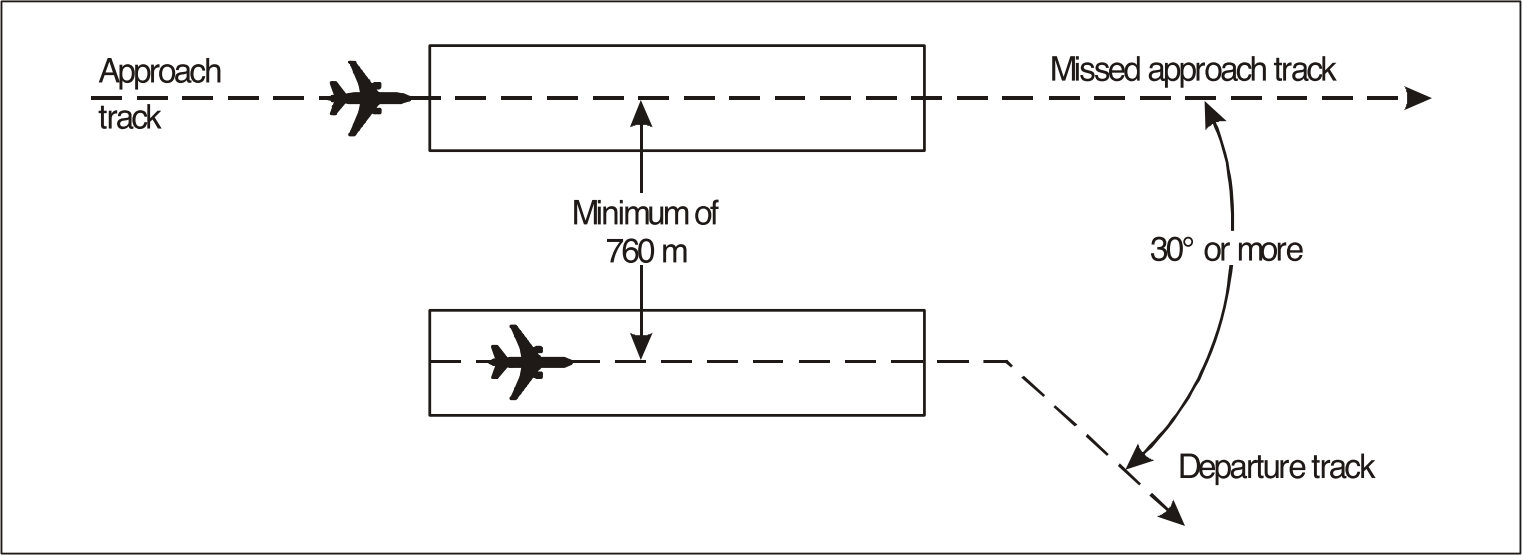
\includegraphics[width=14cm]{Images/Fig 6-1.png}
        \caption[Segregated parallel operations]{Segregated parallel operations (see \ref{6.7.3.5.1} \ref{6.7.3.5.1b})}
        \label{fig:6-1}
    \end{figure}

    \vfill
    \begin{figure}[!ht]
        \centering
        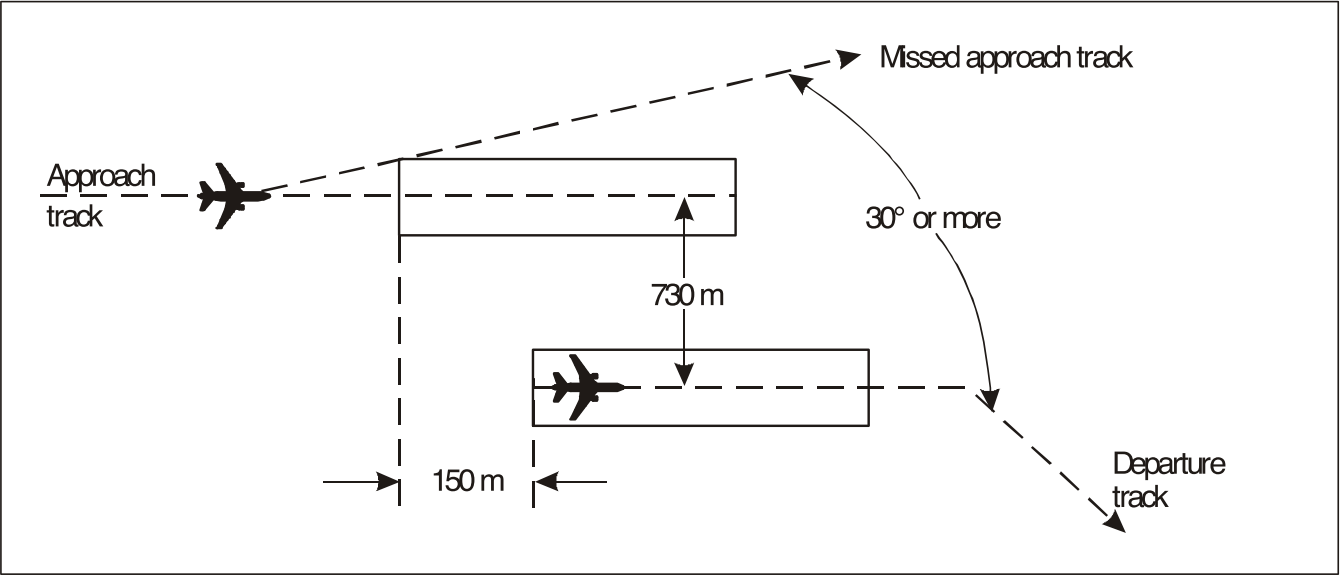
\includegraphics[width=14cm]{Images/Fig 6-2.png}
        \caption[Segregated parallel operations where runways are staggered]{Segregated parallel operations where runways are staggered (see \ref{6.7.3.5.2})}
        \label{fig:6-2}
    \end{figure}

    \vfill
    \begin{figure}[!ht]
        \centering
        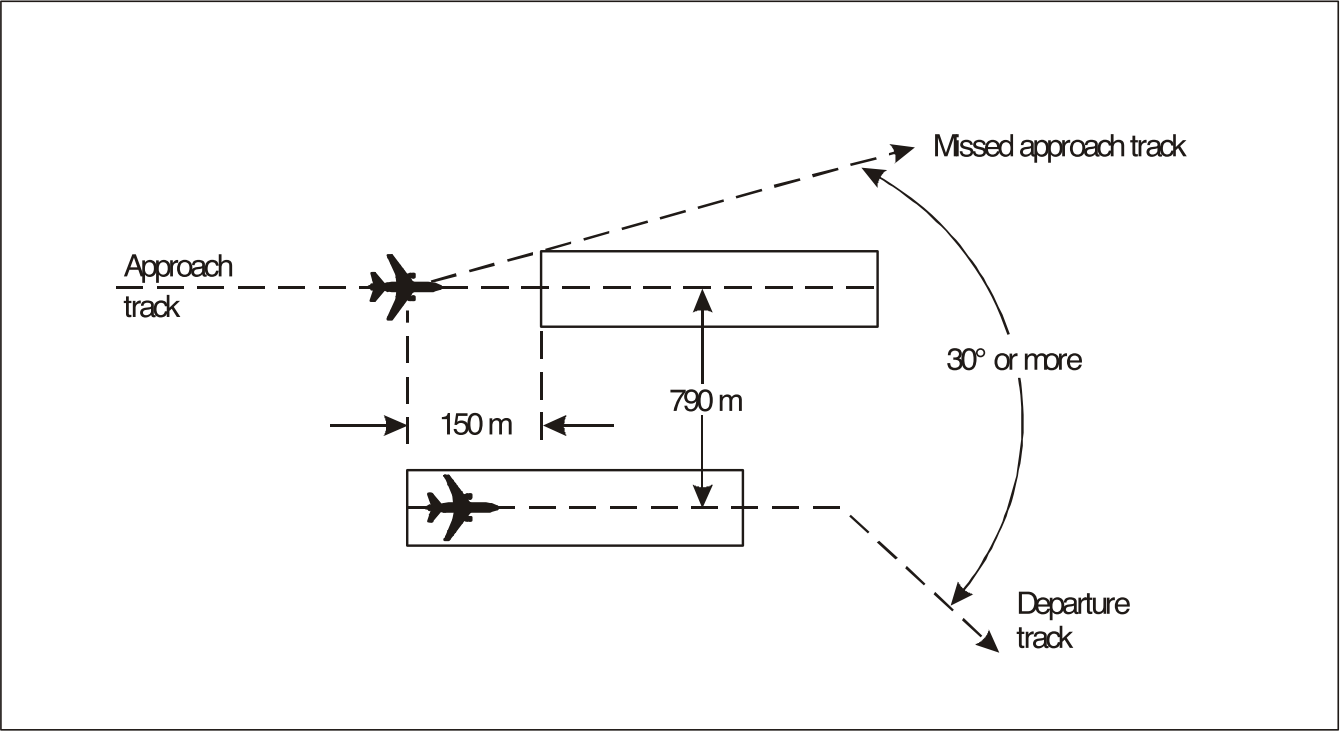
\includegraphics[width=14cm]{Images/Fig 6-3.png}
        \caption[Segregated parallel operations where runways are staggered]{Segregated parallel operations where runways are staggered (see \ref{6.7.3.5.2})}
        \label{fig:6-3}
    \end{figure}

    \newpage

\end{document}
